\section{Filter design}
In this section the process of designing digital filter are described. There will be a distinguished between techniques for IIR and FIR filters..\\
As described ideal filters are not computable hence the process of designing a filter is based on approximation of the frequency response made by computable polynomials.  


\subsection{IIR filter}
One common way of designing an IIR-filter is to design the discrete-time filter from a corresponding continuous-time system. The idea follows four main steps. 
\begin{itemize}
\item[1.] Specify the properties desired for the filter.
\item[2.] Hereby compute a "prototype" by a continuous-time system $H_c(j\Omega)$ that approximates the given properties.
\item[3.] Transform the "prototype" into the discrete-time filter $H(e^{j\omega})$ by...
\item[4.] Implementation of the filter. 
\end{itemize}
The properties of a system are specified on behave of the desired application, considering what frequencies are to pass the filter ideally. Further it is important to specify how much the filter are allowed to vary from the ideal properties, from which it will vary. \\
Properties for an approximation to a lowpass filter could be defined by bounding the magnitude within $\pm \ \delta_1$ of unity in a limited frequency band $0 \leq \Omega \leq \Omega_p $ and less than $\delta_2$ in the frequency band $\Omega_s \leq \Omega$\trine{beskrivelse af convertering af spec. er udkommenteret}. 
The tolerance scheme pleasing the continuous-time filter is illustrated on figure \ref{fig:scheme}\\ 
The transition off nonzero width between the cutoff frequency of passband and stopband is necessary in order for the system to be realizable.

\begin{figure}[H]
\centering
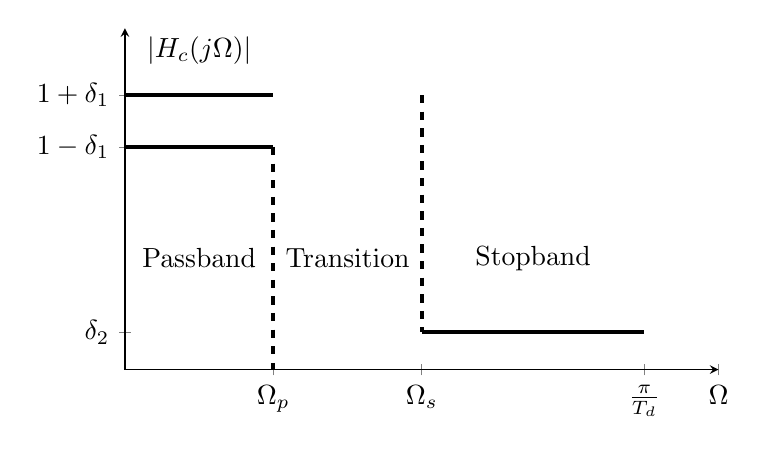
\begin{tikzpicture}[scale=1]
\begin{axis}[
scale=1.1,
unit vector ratio*=1 1 1,
axis lines = middle,
xtick={0,2,4,7,8},
xticklabels={$0$,$\Omega_p$,$\Omega_s$,$\frac{\pi}{T_d}$,$\Omega$},
ytick={0.5,3,3.7},
yticklabels={$\delta_2$,$1-\delta_1$,$1+\delta_1$},
xmin=0,
xmax=8,
ymin=0,
ymax=4.6]
\node at (axis cs:1,4.3) {$|H_c(j\Omega)|$};
\draw[line width=0.5mm](axis cs:0,3.7)--(axis cs:2,3.7);
\draw[line width=0.5mm](axis cs:0,3)--(axis cs:2,3);
\draw[line width=0.5mm, dashed](axis cs:2,3)--(axis cs:2,0);
\draw[line width=0.5mm, dashed](axis cs:4,3.7)--(axis cs:4,0.5);
\draw[line width=0.5mm](axis cs:4,0.5)--(axis cs:7,0.5);
\node at (axis cs:1,1.5) {Passband};
\node at (axis cs:3,1.5) {Transition};
\node at (axis cs:5.5,1.5) {Stopband};
\end{axis}
\end{tikzpicture}
\caption{Specification of frequency response}
\label{fig:scheme}
\end{figure}

Methods for defining a continuous-time system that fits the specification are establish as known continuous-time filter designs. The \textit{Butterworth filter} which is a lowpass filter approximation will now be described along with the Bbiliniare transformation.\\
For a Butterworth filter the squared magnitude are defined as follows.
\begin{align}\label{eq:butter}
|H_c(j\Omega)|^2=\frac{1}{1+\left( \frac{j\Omega}{j\Omega_c}\right)^{2N}}
\end{align} 
Further the filter is characterised by the following three properties.
\begin{align}
1.& \ \ \ |H_c(j\Omega)|^2 = 1 \  \ \left|\begin{matrix}
\\ 
\Omega=0
\end{matrix}\right. , \textit{ for all }N. \\
2.& \ \ \ |H_c(j\Omega)|^2 = \frac{1}{2} \  \ \left|\begin{matrix}
\\ 
\Omega=\Omega_c
\end{matrix}\right. , \textit{ for all }N. \\
3.& \ \ \ \textit{Magnitude response is monotonic in pass- and stopband.}
\end{align}
As the order $N$ of the filter increases the characteristics become sharper and the filter approximates the ideal lowpass filter. This is illustrated on figure \ref{fig:butter}. By\eqref{eq:butter} it is possible to compute the order necessary for the system to fulfil the specifications.            
\begin{figure}[H]
    \centering
    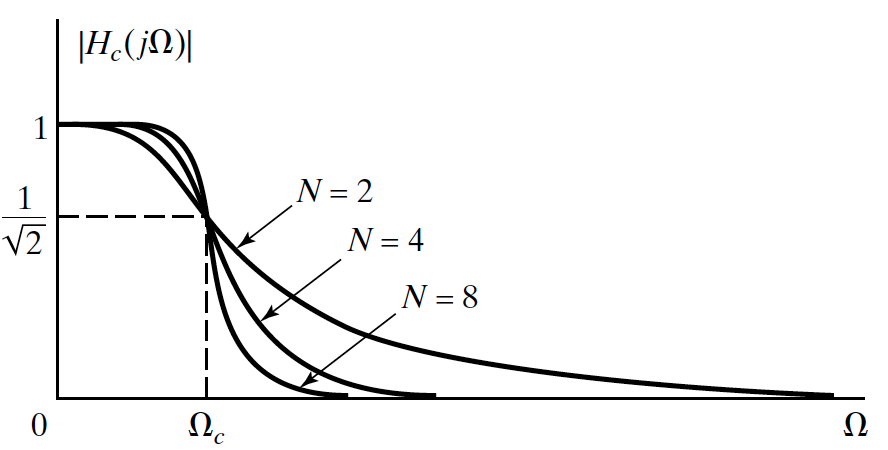
\includegraphics[width = 0.6\textwidth]{figures/butterworth.png}
    \caption{Magnitude of Butterworth filter depending on order $N$ }
    \label{fig:butter}
\end{figure} 
In order to obtain causality and stability in the system representation in the $s$-domain is wanted. By substituting $s=j\Omega$ the following relation is true.
\begin{align}
|H_c(j\Omega)|^2 = H_c(s)H_c(-s)= \frac{1}{1+\left( \frac{s}{j\Omega_c}\right)^{2N}}
\end{align} 
By letting the denominator in \eqref{eq:butter} equal to zero it is possible to determine the poles $s_k$ of the system as 
\begin{align}
s_k = (-1)^{\frac{1}{2N}}\left(j\Omega_c\right)=\Omega_c\text{e}^{\left(\frac{j\pi}{2N}\right)\left(2k+N-1\right)}, \ \ k=0,1,\ ... \ , 2N-1 
\end{align}   
The poles will placed equally along the circle of radius $\Omega_c$ as illustrated on figure \ref{??}. By only considering the poles in the left half plane $H_c(s)$ can be construed as a stable system. 
\begin{align}
H_c(s)=\frac{1}{\prod_{k=1}^{N}(s-s_k)}
\end{align}    
When the continuous-time filter $H_c(s)$ is defined the next step is the transformation from continuous-time to discrete-time. The bilinear transformation is a method that allows a direct transformation between the s- and z-domain. The principal of the transformation is that the imaginary axis $j\Omega$ of the s-plane is mapped onto the z-plane as the unitcircle. The bilinear transformation is defined by 
\begin{align}
s=\frac{2}{T_d}\left(\frac{1-z^{-1}}{1+z^{-1}}\right) 
\end{align}
such that 
\begin{align}
H_c\left[\frac{2}{T_d}\left(\frac{1-z^{-1}}{1+z^{-1}}\right)\right]=H_c(z), 
\end{align}  
Because $-\infty \leq \Omega \leq \infty $ is mapped to $-\pi \leq \omega \leq \omega$ the transformation is non linear which involves some frequency distortion. By this the method is restricted to situations where this is acceptable or can be compensated. Compensation can be done by the concept of pre wrapping, that consider the relation 
\begin{align}
\Omega_{c_{new}}=\frac{2}{T_d}\tan\frac{\omega_c}{2}
\end{align}
hereby it is possible to determine a new $\Omega_c$ to the continuous-time filter, in order to ensure the discrete $\omega_c$ to fit the specification.\\
An important property of the bilinear transformation is that stability is preserved if the continuous-time filter i stable. 
... \\
Advantages of IIR filter:
The process of designing a IIR filter is are rather simple when the desired properties fits an establish design method such as Butterworth. The required order of the filter is computable and the transformation to the discrete-time domain is to be done straight forward by design equations. Thus, considering the implementation, this leads to non iterative algorithms. \\
Though by this method the magnitude response is the only parameter to be specified. Meaning that specific requirements for e.g. phase response or group delay are quarantined not to be fulfilled by this kind of IIR filter. \\
\\
If the desired specifications of a system are appropriate for a establish design method such as Butterworth, the required order can be computed and the transformation can be done straightforward by 
     

%
%These properties are to be converted into specifications of the discrete-time filter by expressing the frequency in normalised radian frequency by the relation $\omega=\Omega T_d$ where $T_d$ is the sampling rate. Thus the impulse response is specified over one period as 
%\begin{align}
%H_c(j\Omega)=H(e^{j\omega}), \ \ |\omega|<\pi
%\end{align}    
%
%The desired gain of the magnitude is often expressed in dB, where $20\log(1)=0[\text{dB}]$ \trine{is gain of magnitude a thing?} \\

Because the analogue frequency response is known it is as described possible to determine the corresponding impulse response, which by sampling can be made discrete whereby the discrete frequency impulse is obtained through the Fourier transformation. Further the  

\subsection{FIR filter}

\subsection{Anti aliasing filter}
As mentioned in section \ref{ADC} an anti aliasing filter is required in the ADC process. The purpose of filter is to avoid the aliasing phenomenon which occurs when the samplings theorem \ref{sampling_theorem} is not fulfilled. As stated a signal has to be band limited by the Nyquist frequency $\omega_N$ and since a continuous-time signal such as a sound is not guaranteed to have a bandlimited frequency the anti aliasing filter is design to remove the frequencies that are above the Nyquist frequency. \\
An anti aliasing filter typically form an analogue low pass filter, with the Nyquist frequency as the ideal cut off frequency. Though as seen a transition band is necessary - when designing a practical filter - in which the frequencies can cause aliasing. This causes the passband cut of frequency to be larger than the Nyquist frequency.\trine{how larger}           